\documentclass[tikz, border=5mm]{standalone}
\usepackage{pgfplots}
\pgfplotsset{compat=1.18}
\usetikzlibrary{calc, arrows.meta}

\begin{document}
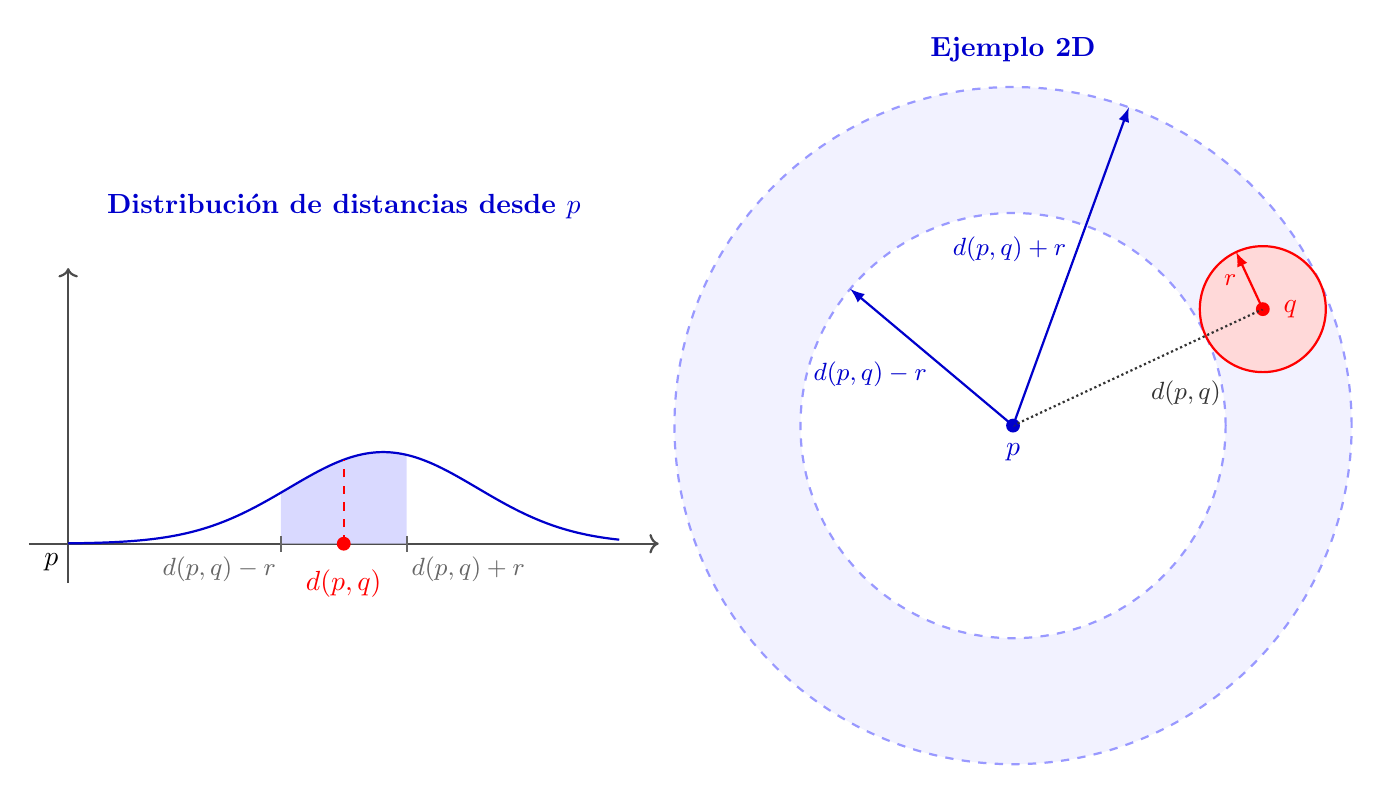
\begin{tikzpicture}

    % --- Parámetros matemáticos globales ---
    \def\dpq{3.5}       % Distancia exacta entre p y q: d(p,q)
    \def\rad{0.8}       % Radio de la consulta q: r
    \def\rmin{\dpq-\rad}% Límite inferior: d(p,q) - r
    \def\rmax{\dpq+\rad}% Límite superior: d(p,q) + r
    
    \def\muP{4.0}       % Media de la gaussiana (distribución de distancias)
    \def\sigmaP{1.2}    % Desviación estándar de la gaussiana

    % Función gaussiana escalada (el multiplicador 3.5 ajusta la altura visual)
    \tikzset{
        declare function={
            gauss(\x,\mu,\sigma)=3.5 * (1/(\sigma*sqrt(2*pi))*exp(-((\x-\mu)^2)/(2*\sigma^2)));
        }
    }


    % =========================================================================
    % PARTE IZQUIERDA: Distribución de distancias relativas al pivote p (1D)
    % =========================================================================
    \begin{scope}[xshift=0cm]
        
        % 1. Ejes
        \draw[->, thick, black!70] (-0.5, 0) -- (7.5, 0) node[right] { };
        \draw[->, thick, black!70] (0, -0.5) -- (0, 3.5) node[above] { };
        \node[below left] at (0,0) {$p$};

        % 2. Sombrear el área de intersección [d(p,q)-r, d(p,q)+r]
        % Representa los elementos que no pueden ser podados (pruning) por p
        \fill[blue!15] (\rmin, 0) 
            -- plot[domain=\rmin:\rmax, samples=50] (\x, {gauss(\x,\muP,\sigmaP)}) 
            -- (\rmax, 0) -- cycle;

        % 3. Dibujar la curva gaussiana principal
        \draw[thick, blue!80!black, smooth, domain=0:7, samples=100] plot (\x, {gauss(\x,\muP,\sigmaP)});

        % 4. Marcar la distancia d(p,q) exacta
        \draw[red, thick, dashed] (\dpq, 0) -- (\dpq, {gauss(\dpq,\muP,\sigmaP)});
        \fill[red] (\dpq, 0) circle (2.5pt) node[below=6pt, font=\bfseries] {$d(p,q)$};

        % 5. Marcar los límites del intervalo en el eje X
        \draw[thick, black!60] (\rmin, 0.1) -- (\rmin, -0.1) node[below left=-2pt, font=\small] {$d(p,q)-r$};
        \draw[thick, black!60] (\rmax, 0.1) -- (\rmax, -0.1) node[below right=-2pt, font=\small] {$d(p,q)+r$};

        % 6. Título de la sección
        \node[above, font=\bfseries, blue!80!black] at (3.5, 4) {Distribución de distancias desde $p$};
        
    \end{scope}


    % =========================================================================
    % PARTE DERECHA: Vista espacial geométrica (2D)
    % =========================================================================
    \begin{scope}[xshift=12cm, yshift=1.5cm]
        
        % 1. Definir el Pivote p en el origen de este scope
        \coordinate (P) at (0,0);
        
        % 2. Definir la Consulta q en un ángulo de 25 grados a distancia \dpq
        \coordinate (Q) at (25:\dpq);

        % 3. Dibujar el anillo de búsqueda (Annulus) centrado en p
        % Usamos 'even odd rule' para rellenar solo el anillo entre rmin y rmax
        \fill[blue!5, even odd rule] (P) circle (\rmax) (P) circle (\rmin);
        \draw[blue!40, thick, dashed] (P) circle (\rmin);
        \draw[blue!40, thick, dashed] (P) circle (\rmax);

        % 4. Dibujar la bola de la consulta (centrada en q con radio r)
        \fill[red!15] (Q) circle (\rad);
        \draw[red, thick] (Q) circle (\rad);

        % 5. Marcar p y q
        \fill[blue!80!black] (P) circle (2.5pt) node[below=3pt, font=\bfseries] {$p$};
        \fill[red] (Q) circle (2.5pt) node[right=4pt, font=\bfseries] {$q$};

        % 6. Vectores y etiquetas de distancias
        % Distancia d(p,q)
        \draw[thick, densely dotted, black!80] (P) -- (Q) node[midway, below right=1pt, font=\small] {$d(p,q)$};
        
        % Radio de la consulta r
        \draw[red, ->, >=latex, thick] (Q) -- ++(115:\rad) node[midway, left=1pt, font=\small] {$r$};

        % Radio interior: d(p,q) - r
        \draw[blue!80!black, ->, >=latex, thick] (P) -- (140:\rmin) node[midway, below left=-2pt, font=\small] {$d(p,q)-r$};
        
        % Radio exterior: d(p,q) + r
        \draw[blue!80!black, ->, >=latex, thick] (P) -- (70:\rmax) node[midway, above left=-2pt, font=\small] {$d(p,q)+r$};

        % 7. Título de la sección
        \node[above, font=\bfseries, blue!80!black] at (0, 4.5) {Ejemplo 2D};

    \end{scope}

    % =========================================================================
    % LÍNEA DIVISORIA (Opcional, para separar visualmente ambas perspectivas)
    % =========================================================================
    %\draw[thick, gray!30, dashed] (8.5, -1.5) -- (8.5, 6.0);

\end{tikzpicture}
\end{document}